\documentclass[final,t]{beamer}
\mode<presentation>{\usetheme{Purdue}}

\usepackage{natbib,url}
\usepackage{multicol}
\usepackage{geometry}
\usepackage{multirow}
\usepackage{rotating}
\usepackage{wrapfig}

\usepackage{tikz}
\usetikzlibrary{shapes,arrows}
\usepackage{graphicx}
\usepackage{tikz-dependency}
\usepackage{natbib}
\usepackage{url}
%\usepackage{gb4e}
\usepackage{amsmath}
\DeclareMathOperator*{\argmax}{arg\,max}
\DeclareMathOperator*{\argmin}{arg\,min}
% MD: This threw an odd error for me:
%\usepackage{tikz-qtree}
\usepackage[framemethod=tikz]{mdframed}

\newcommand{\myboxedtext}[2][rectangle,draw,rounded corners]{%
            \tikz[baseline=-0.6ex] \node [#1,rounded corners]{#2};}%

\usepackage{enumerate}
\usepackage{color}
\usepackage{xcolor}
\usepackage{caption}
\setbeamerfont{caption}{size=\normalsize}

\definecolor{light-gray}{gray}{0.9}
\definecolor{forestgreen}{rgb}{0.13, 0.55, 0.13}
\definecolor{carnelian}{rgb}{0.7, 0.11, 0.11}
\definecolor{darkblue}{rgb}{0.0, 0.0, 0.55}
\definecolor{darkgreen}{rgb}{0.0, 0.2, 0.13}
\definecolor{persimmon}{rgb}{0.93, 0.35, 0.0}

\usepackage[size=custom,width=120,height=90,scale=1]{beamerposter}
\usepackage{gb4e}

\title[]{Annotating Picture Description Task Responses for Content Analysis}
\author[]{Levi King \& Markus Dickinson}
\institute[]{Indiana University}
\date[]{5 June 2018}
\newcommand{\myimg}{
  \framebox{
   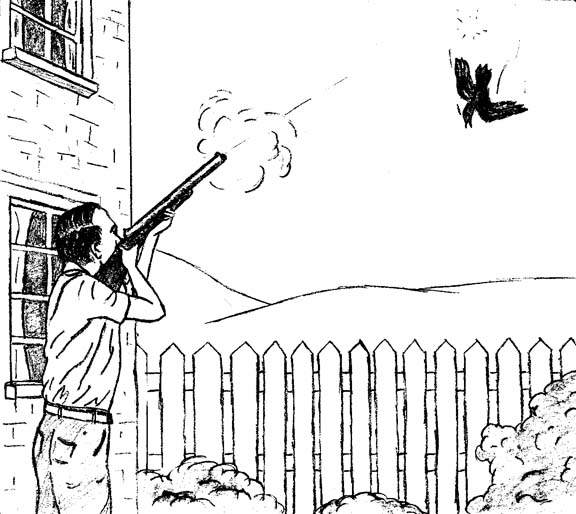
\includegraphics[width=.95\textwidth]{../figures/exampleprompt2.jpg}}}
\setbeamertemplate{caption}[numbered]
\setbeamertemplate{itemize/enumerate body begin}{\normalsize}
\setbeamertemplate{itemize/enumerate subbody begin}{\normalsize}
\setbeamertemplate{itemize/enumerate subsubbody begin}{\normalsize}

\begin{document}
\begin{frame}{}
  \begin{columns}[t]
    \begin{column}{.33\linewidth}

\begin{block}{Overview \& Background}
\begin{center}
\begin{minipage}{.85\textwidth}

  \begin{itemize}
    \itemsep1em
  \item{Introducing the \textbf{Semantic Analysis of Image-based Learner Sentences (SAILS) Corpus}
   \begin{itemize}
  \item 13,533 picture description task (PDT) responses from native speakers (NS) and non-native speakers (NNS), each annotated for five binary features
      \end{itemize}
    }
\end{itemize}
  \begin{itemize}
    \itemsep1em
  \item{\textbf{Goal:} Evaluate content of NNS sentences 
      \begin{itemize}
      \item Compare to gold standard (GS) of NS sentences
      \end{itemize}
    }
\end{itemize}
  
  \begin{itemize}
    \itemsep1em
  \item{\textbf{Needs:}  Adequate data, appropriately constrained
        \begin{itemize}
      \item Large set of PDT responses from NS and NNS participants
      \item Varied task prompts and participant demographics allowing for study of variability
      \item Annotation allowing for content analysis
      \end{itemize}
    }
\end{itemize}

\end{minipage}
\end{center}
\end{block}

\begin{block}{Picture Description Task}
\begin{center}
\begin{minipage}{.85\textwidth}

	\vspace{-.38em}
    \begin{itemize}
    \item{PDT elicits natural productions but constrains form \& content}
    \item{60 \textbf{items}: 30 images $x$ 2 prompts}
    \begin{itemize}
    \item 30 images
    \begin{itemize}
    	\item simple vector graphics
		\item 10 transitive, 10 intransitive, 10 ditransitive actions
	\end{itemize}
    \item 2 prompt versions:
    	\begin{itemize}
			\item \textbf{targeted}: \textit{What is $<$the subject$>$ doing?}
			\item \textbf{untargeted}: \textit{What is happening?}
		\end{itemize}
	\end{itemize}
    \end{itemize}
	\bigskip
\setlength{\fboxsep}{3pt}
\setlength{\fboxrule}{0pt}
\begin{table}[htb!]
\begin{center}
\begin{tabular}{|c|c|c|}
\hline
Intransitive & Transitive & Ditransitive \\
\hline
{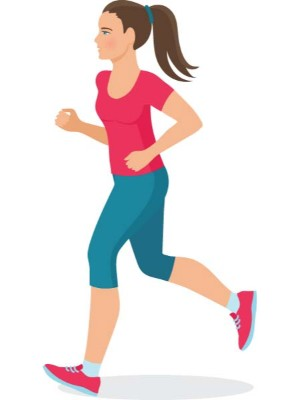
\includegraphics[width=0.29\columnwidth]{../figures/I30.jpg}} & {
\includegraphics[width=0.3\columnwidth]{../figures/I29.jpg}} & {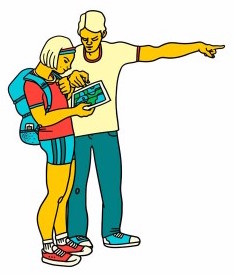
\includegraphics[width=0.3\columnwidth]{../figures/I28.jpg}} \\
What is the woman doing? & What is the woman doing? & What is the man doing? \\
\hline
%\hline
%{
\includegraphics[width=0.29\columnwidth]{../figures/I20.jpg}} & {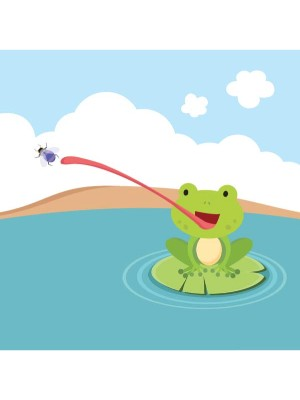
\includegraphics[width=0.3\columnwidth]{../figures/I16.jpg}} & {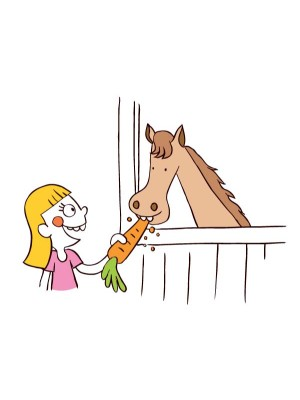
\includegraphics[width=0.3\columnwidth]{../figures/I17.jpg}} \\
%What is the girl doing? & What is the frog doing? & What is the girl doing? \\
%\hline
\end{tabular}
\medskip
\caption{\label{tab:example-pdt-items} Example PDT images with their \textbf{targeted} questions. In the \textbf{untargeted} form, the question for each is \textit{What is happening?}} %From left to right, the examples represent two intransitive, transitive and ditransitive items.}
\end{center}
\end{table}

\begin{itemize}
	\item PDT Instructions: Focus on main action; Respond with complete sentence
%	\begin{itemize}
%		\item Focus on the main action
%		\item Respond in a complete sentence
%	\end{itemize}
	\item Task administered as online survey (SurveyMonkey.com)
	\item Multiple versions
	\begin{itemize}
		\item Most participants completed 30 items
		\item Roughly equal number of targeted \& untargeted responses collected per image
		\item NNSs provide one response per item
		\item NSs asked to provide two non-identical responses per item
		\begin{itemize}
			\item Intended to increase variety of NS responses for a more robust GS
		\end{itemize}
	\end{itemize}
\end{itemize}

\end{minipage}
\end{center}
\vspace{-.5em}
\end{block}


\begin{block}{Participants}

\begin{center}
\begin{minipage}{.85\textwidth}
499 total participants
	\begin{itemize}
		\item 141 NNSs
		\begin{itemize}
%			\item Recruited from intermediate \& advanced English as a Second Language writing courses at Indiana University
			\item Recruited from intermediate \& advanced ESL writing courses at Indiana University
			%\item Performed task in computer lab with researchers present
			\item L1s: 125 Chinese (90\%), 4 Korean, 3 Burmese, 2 Hindi; 1 each: Arabic, Indonesian, German, Gujarati, Spanish, Thai, Vietnamese
		\end{itemize}
		\item 358 NSs
		\begin{itemize}
			%\item All NSs performed task remotely
			\item 29 Familiar Native Speakers (FNSs)
			\begin{itemize}
				\item Relatives or friends of researchers; assumed to be high quality
%				\item Responses are assumed to be high quality
			\end{itemize}
			\item 329 Crowdsourced Native Speakers (CNSs)
			\begin{itemize}
				\item Responses purchased via SurveyMonkey; assumed to be lower quality
				%\item Limited by SurveyMonkey to only 15 items per participant
%				\item Responses are assumed to be lower quality
			\end{itemize}
		\end{itemize}
	\end{itemize}
\end{minipage}
\end{center}
\vspace{-.5em}
\end{block}
\end{column}

\begin{column}{.33\linewidth}

\begin{block}{Responses}
\begin{center}
\begin{minipage}{.85\textwidth}

The SAILS Corpus contains a total of 13,533 PDT responses.
\vspace{.5em}
\begin{table}[htb!]
\begin{center}
\begin{tabular}{|l||r|r||r|}
\hline
& \multicolumn{3}{|c|}{Response Counts} \\
\hline
 Group & First & Second & Total \\
\hline
\hline
NNS & 4290 & 0 & 4290 \\
\hline
\hline
NS (all) & 4634 & 4609 & 9243 \\ 
\hline
\multicolumn{1}{|r||}{FNS} & 642 & 641 & 1283 \\ 
\hline
\multicolumn{1}{|r||}{CNS} & 3992 & 3968 & 7960 \\
\hline
\hline
Total & 8924 & 4609 & 13,533 \\
\hline
\end{tabular}
\caption{\label{tab:response-counts} First and second response counts for the SAILS Corpus participant groups. Familiar (FNS) and crowdsourced (CNS) are subgroups of NS. NNS participants are not asked to provide a second response.}
\end{center}
\end{table}

\vspace{1em}
In order to examine the level of variation among responses, type to token ratios (TTRs) were calculated on the response level. Capitalization and final punctuation were ignored. We can see that variation increases with item complexity (intransitives $<$ transitives $<$ ditransitives) and that untargeted responses vary more than targeted responses.
\vspace{.5em}
\begin{table}[h!]
\begin{center}
\begin{tabular}{|l||l|l||l|l|}
\hline
 & \multicolumn{2}{|c||}{Targeted} & \multicolumn{2}{|c|}{Untargeted} \\
\hline
 Set & NS & NNS & NS & NNS \\
\hline
\hline
Intransitives & 0.628 & 0.381 & 0.782 & 0.492 \\
\hline
Transitives & 0.752 & 0.655 & 0.859 & 0.779 \\
\hline
Ditransitives & 0.835 & 0.817 & 0.942 & 0.936 \\ 
\hline
\end{tabular}
\caption{\label{tab:ttr} NS and NNS type-to-token ratios (TTR) for complete responses (not words), for the full corpus.}
\end{center}
\end{table}

\vspace{1em}
TTRs were also calculated to compare the variability among NSs' first responses versus their second responses. As the TTRs for second responses are considerably higher than those for first responses, asking for two non-identical responses appears to effectively increase the variety of NS responses available for use in a GS.
\vspace{.5em}
\begin{table}[hb!]
\begin{center}
\begin{tabular}{|l||l|l||l|l|}
\hline
 & \multicolumn{2}{|c||}{Targeted} & \multicolumn{2}{|c|}{Untargeted} \\
\hline
 Set & R1 & R2 & R1 & R2 \\
\hline
\hline
Intransitives & 0.343 & 0.819 & 0.549 & 0.939 \\
\hline
Transitives & 0.509 & 0.895 & 0.682 & 0.926 \\
\hline
Ditransitives & 0.641 & 0.948 & 0.864 & 0.955  \\ 
\hline
\end{tabular}
\caption{\label{tab:ttr1v2} TTRs for complete responses, separated by first responses (R1) and second responses (R2). The ratios here are calculated from all NS responses; NNS responses are not included.}
\end{center}
\end{table}

\end{minipage}
\end{center}
\vspace{-.5em}
\end{block} 

\begin{block}{Annotation Scheme}
\begin{center}
\begin{minipage}{.85\textwidth}
Two annotators:
\begin{itemize}
	\item NSs (US English), both with language teaching experience (child \& adult learners).
	\item Annotator 1 (A1) annotated the complete corpus, Annotator 2 (A2) annotated development set \& test set, each containing 1 intransitive, 1 transitive, 1 ditransitive.
\end{itemize}
\vspace{1em}

Initial scheme (\textit{accurate $+$ native-like} $>$ \textit{accurate $+$ not native-like} $>$ \textit{not accurate}) proved problematic; evolved to five binary features related to accuracy \& native-likeness.
\vspace{.5em}
\begin{enumerate}
\item \textbf{Core Event}: Does the response capture the core event depicted in the image?
%Core events are not pre-defined for annotators but should be obvious given the nature of the images. The response should link an appropriate subject to the event.  In Table~\ref{tab:sample-responses}, \textit{[The woman is] holding a puppy and looks happy} clearly captures the core event, while \textit{She is wear a blue dress} is irrelevant to the event happening.
\vspace{.5em}
\item \textbf{Verifiability}: Does the response contain only information that is true and verifiable based on the image? Inferences allowed only when necessary; e.g., familial relationships between persons in image. 
%For example, in Table~\ref{tab:sample-responses}, \textit{She is wear a blue dress} conveys information that is irrelevant to the core event but is nonetheless recoverable from the image (core event=0, verifiability=1), while \textit{hugging her dog Fluffy that she missed while on vacation} fulfills the core event but also has information that cannot be inferred from the picture (core event=1, verifiability=0).
\vspace{.5em}
\item \textbf{Answerhood}: Does the response make a clear attempt to answer the question? This generally requires a progressive verb. For targeted items, the subject of the question or an appropriate pronoun must be used as the subject of the response.
%For example, \textit{The dog is so happy!} is answering a question other than \textit{What is the woman doing?}. 
\vspace{.5em}
\item \textbf{Interpretability}: Does the response evoke a clear mental image (even if different from the actual item image)? Any required verb arguments must be present and unambiguous.
%For example, \textit{She loves her pet} is too vague to generate a clear mental image. No action is specified (unless we force an unlikely reading of \textit{loves} as a dynamic, simple present verb), and we cannot know if the \textit{pet} is a dog, a horse, etc.
\vspace{.5em}
\item \textbf{Grammaticality}: Is the response free from errors of spelling and grammar?  
%In the SAILS responses, this is a relatively straightforward feature to annotate. For example, from Table~\ref{tab:sample-responses}, \textit{She is wear a blue dress} contains an ungrammatical verb form.

\end{enumerate}



\end{minipage}
\end{center}
\vspace{-.5em}
\end{block}

\end{column}

\begin{column}{.33\linewidth}
\vspace{-1em}
\begin{block}{Annotation Results}
\begin{center}
\begin{minipage}{.85\textwidth}

%\begin{table}[htb!]
%\begin{center}
%\begin{tabular}{|l|c|c|c|c|c|}
%\hline
%\multicolumn{6}{|c|}{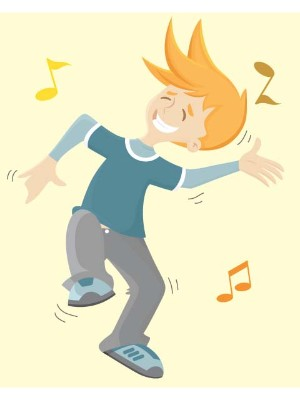
\includegraphics[width=0.29\columnwidth]{../figures/I01.jpg}} \\ 
%\hline
%\textit{What is the boy doing?} (Targeted) & C & V & A & I & G \\
%\hline
%\hline
%eating food. & 0 & 1 & 1 & 1 & 1 \\
%\hline
%eatting. & 0 & 1 & 1 & 1 & 0 \\
%\hline
%The child is about to eat pizza. & 1 & 1 & 0 & 1 & 1 \\
%\hline
%He may get fat eating pizza. & 1 & 0 & 0 & 1 & 1 \\
%\hline
%\hline
%\hline
%\textit{What is happening?} (Untargeted) & C & V & A & I & G \\
%\hline
%\hline
%Child is eating pizza. & 1 & 1 & 1 & 1 & 0 \\
%\hline
%Tommy is eating pizza. & 1 & 0 & 1 & 1 & 1 \\
%\hline
%The boy's eating his favorite food. & 0 & 0 & 1 & 0 & 1 \\
%\hline
%Pizza is this boy's favorite food. & 0 & 0 & 0 & 0 & 1 \\
%\hline
%\end{tabular}
%\caption{\label{tab:devo-transitive} Sample responses from the development set transitive item, shown with adjudicated annotations for the five features: core event (\textit{C}), verifiability (\textit{V}), answerhood (\textit{A}), interpretability (\textit{I}) and grammaticality (\textit{G}).}
%\end{center}
%\end{table}

\begin{table}[htb!]
\begin{center}
\begin{tabular}{|l||l|c|c|c|c|c|}
\hline
\multirow{10}{*}{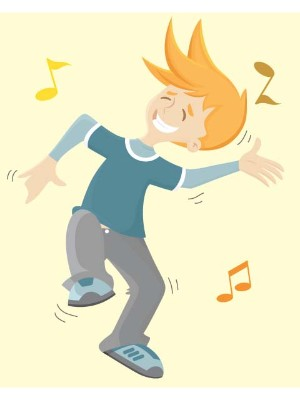
\includegraphics[width=0.25\columnwidth]{../figures/I01.jpg}}& \textit{What is the boy doing?} (Targeted) & C & V & A & I & G \\
\cline{2-7}
\cline{2-7}
& eating food. & 0 & 1 & 1 & 1 & 1 \\
\cline{2-7}
& eatting. & 0 & 1 & 1 & 1 & 0 \\
\cline{2-7}
& The child is about to eat pizza. & 1 & 1 & 0 & 1 & 1 \\
\cline{2-7}
& He may get fat eating pizza. & 1 & 0 & 0 & 1 & 1 \\
\cline{2-7}
& \multicolumn{6}{c|}{} \\
\cline{2-7}
& \textit{What is happening?} (Untargeted) & C & V & A & I & G \\
\cline{2-7}
\cline{2-7}
& Child is eating pizza. & 1 & 1 & 1 & 1 & 0 \\
\cline{2-7}
& Tommy is eating pizza. & 1 & 0 & 1 & 1 & 1 \\
\cline{2-7}
& The boy's eating his favorite food. & 0 & 0 & 1 & 0 & 1 \\
\cline{2-7}
& Pizza is this boy's favorite food. & 0 & 0 & 0 & 0 & 1 \\
\hline
\end{tabular}
\caption{\label{tab:devo-transitive} Sample responses from the development set transitive item, shown with adjudicated annotations for the five features: core event (\textit{C}), verifiability (\textit{V}), answerhood (\textit{A}), interpretability (\textit{I}) and grammaticality (\textit{G}).}
\end{center}
\end{table}

%\begin{table}[htb!]
%\begin{center}
%\begin{tabular}{|l|c|c|c|c|c|c|l|c|c|c|c|c|}
%\hline
%\multicolumn{13}{|c|}{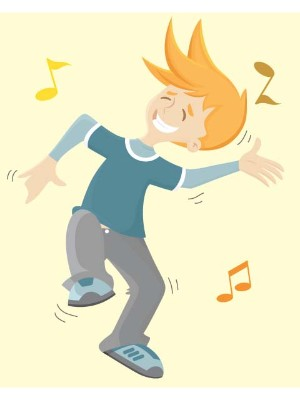
\includegraphics[width=0.29\columnwidth]{../figures/I01.jpg}} \\ 
%\hline
%\textit{What is the boy doing?} & C & V & A & I & G && \textit{What is happening?} & C & V & A & I & G \\
%\hline
%\hline
%eating food. & 0 & 1 & 1 & 1 & 1 && Child is eating pizza. & 1 & 1 & 1 & 1 & 0 \\
%\hline
%eatting. & 0 & 1 & 1 & 1 & 0 && Tommy is eating pizza. & 1 & 0 & 1 & 1 & 1 \\
%\hline
%The child is about to eat pizza. & 1 & 1 & 0 & 1 & 1 && The boy's eating his favorite food. & 0 & 0 & 1 & 0 & 1 \\
%\hline
%He may get fat eating pizza. & 1 & 0 & 0 & 1 & 1 && Pizza is this boy's favorite food. & 0 & 0 & 0 & 0 & 1 \\
%\hline
%\end{tabular}
%\caption{\label{tab:devo-transitive} Targeted and untargeted sample responses shown with adjudicated annotations for the development set transitive item (see Table~\ref{tab:example-pdt-items}).}
%\end{center}
%\end{table}

\vspace{1em}
Using the items shown in Table~\ref{tab:example-pdt-items}, we calculated inter-annotator agreement for each feature, for targeted vs. untargeted items, and for the three verb types.
%, as shown in Table~\ref{tab:agreement}. 
\vspace{1em}
\begin{table}[htb!]
\begin{center}
\begin{tabular}{|l|l|l|l|l||l|l||l|}
\hline
Set	& Total	& A1Yes & A2Yes & AvgYes & Chance & Agree & Kappa \\
\hline
\hline
Intransitive & 2155 & 0.863 & 0.855 & 0.859 & 0.758 & 0.978 & 0.910 \\
\hline
Transitive & 2155 & 0.780 & 0.774 & 0.777 & 0.653 & 0.949 & 0.853 \\
\hline
Ditransitive & 2155 & 0.812 & 0.786 & 0.799 & 0.678 & 0.924 & 0.764 \\ 
\hline
\hline
Targeted & 3390 & 0.829 & 0.818 & 0.824 & 0.709 & 0.949 & 0.823 \\
\hline
Untargeted & 3075 & 0.806 & 0.790 & 0.798 & 0.678 & 0.952 & 0.872 \\
\hline
\hline
Core Event & 1293 & 0.733 & 0.717 & 0.725 & 0.601 & 0.923 & 0.808 \\
\hline
Verifiability & 1293 & 0.845 & 0.817 & 0.831 & 0.719 & 0.968 & 0.884 \\
\hline
Answerhood & 1293 & 0.834 & 0.831 & 0.833 & 0.721 & 0.982 & 0.936 \\
\hline
Interpretability & 1293 & 0.818 & 0.787 & 0.802 & 0.682 & 0.919 & 0.744 \\
\hline
Grammaticality & 1293 & 0.861 & 0.872 & 0.866 & 0.768 & 0.960 & 0.827 \\
\hline
\end{tabular}
\caption{\label{tab:agreement} Agreement scores broken down by different properties of the test set: total annotations (\textit{Total}), \textit{yes} annotations for Annotator 1 and 2 (\textit{A1Yes}, \textit{A2Yes}), average \textit{yes} annotations (\textit{AvgYes}), total expected chance agreement for \textit{yes}es and \textit{no}s (\textit{Chance}), actual raw agreement (\textit{Agree}) and Cohen's kappa (\textit{Kappa}).}
\end{center}
\end{table}
\vspace{1em}

Observations from Table~\ref{tab:agreement}:
\begin{itemize}
	\vspace{.5em}
	\item Average \textit{yes} rates are included to show that all features skew toward \textit{yes} annotations; Cohen's kappa is thus used as a measure of inter-annotator agreement;
	\vspace{.5em}
	\item Cohen's kappas well above the conventional 0.67 threshold for meaningful agreement, so we believe the annotation scheme can be implemented reliably by following the guidelines;
	\vspace{.5em}
	\item Inter-annotator agreement decreases with item complexity, from intransitive to transitive to ditransitive verbs;
	\vspace{.5em}
	\item Agreement is slightly higher for untargeted items than targeted items, likely due to the fact that annotation guidelines are less complicated for untargeted items;
	\vspace{.5em}
	\item Among the features, answerhood has the highest kappa and interpretability has the lowest. This is unsurprising, as annotators reported these to be the easiest and hardest features to annotate, respectively.
\end{itemize}

\end{minipage}
\end{center}
\end{block}

\begin{block}{Accessing the SAILS Corpus}
The entire annotated SAILS Corpus, the PDTs and annotation guidelines are available to anyone at:

\vspace{.5em}
\textbf{https://github.com/sailscorpus/sails}

\vspace{.5em}
We believe the corpus can be a useful resource for language testing and ICALL, as well as other areas of research like question answering, dialog systems, pragmatic modeling, and visual references. We hope that other researchers will make use of the existing data or expand on it with new participants, items, and approaches for processing.

\end{block}

\end{column}

\end{columns}
\end{frame}
\end{document}